\documentclass[11pt, a4paper]{article}
\usepackage[UTF8, heading=true]{ctex}
\usepackage[dvipsnames, x11names]{xcolor}
\usepackage{geometry}
\usepackage{subcaption}
\usepackage{float}
\usepackage{graphicx}
\usepackage{listings}

\newfontfamily\codefont{Cascadia Code}
\definecolor{codebackground}{RGB}{230 235 245}

\lstset{
    basicstyle          =   \small\codefont,
    % ---
    tabsize             =   4,
    showstringspaces    =   false,
    numbers             =   left,
    numberstyle         =   \codefont,
    % ---
    breaklines          =   true,
    captionpos          =   t,      
    % ---
    frame               =   l,
    flexiblecolumns,
}

\lstdefinestyle{python}{
    language        =   Python, % 语言选Python
    keywordstyle    =   \bfseries\color{blue},
    % keywordstyle    =   [2] \color{teal},
    stringstyle     =   \color{orange!80!black},
    commentstyle    =   \color{OliveGreen},
    % identifierstyle =   \color{blue!80!white},
    backgroundcolor =   \color{codebackground}
}

\geometry{a4paper, scale=0.8}

\ctexset{
    section = {
        name = {第,题},
        format = {\Large\bfseries}
    }
}

\title{\Large{\bf{视听信息系统导论编程1}}}
\author{高艺轩\ 毕嘉仪}
\date{}

\begin{document}
\maketitle
\section{}
在SGD优化器下,输出的结果如下:
\begin{figure}[H]
    \hfill
    \begin{subfigure}[t]{0.45\linewidth}
        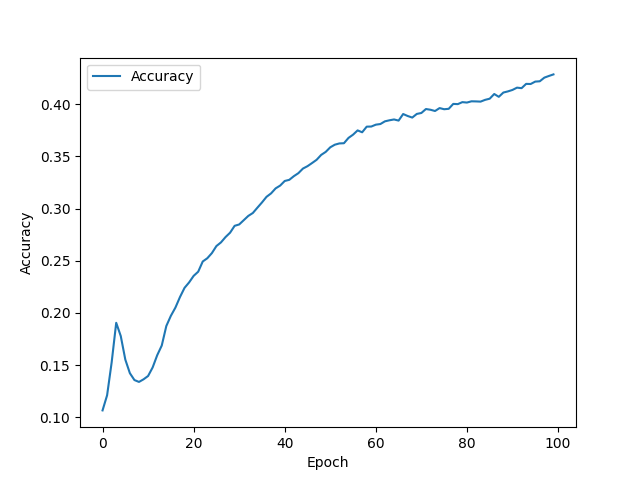
\includegraphics[width=\textwidth]{img/Q1/Acc.png}
    \end{subfigure}
    \hfill
    \begin{subfigure}[t]{0.45\linewidth}
        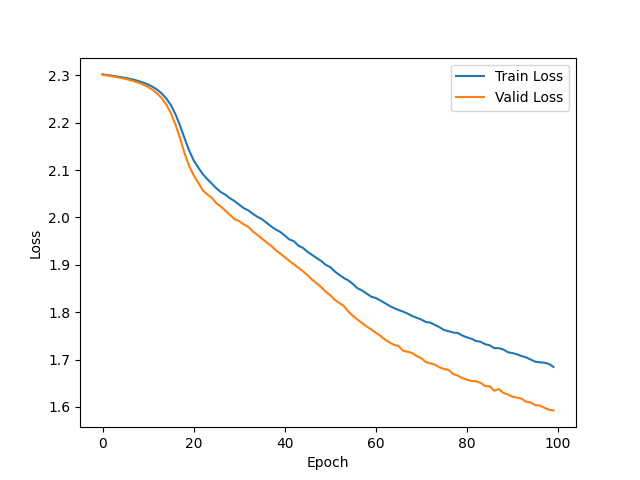
\includegraphics[width=\textwidth]{img/Q1/Loss.png}
    \end{subfigure}
    \hfill
\end{figure}

\section{}
在SGD优化器下,使用ReLU激活函数与Batch Normalization,输出的结果如下:
\begin{figure}[H]
    \hfill
    \begin{subfigure}[t]{0.45\linewidth}
        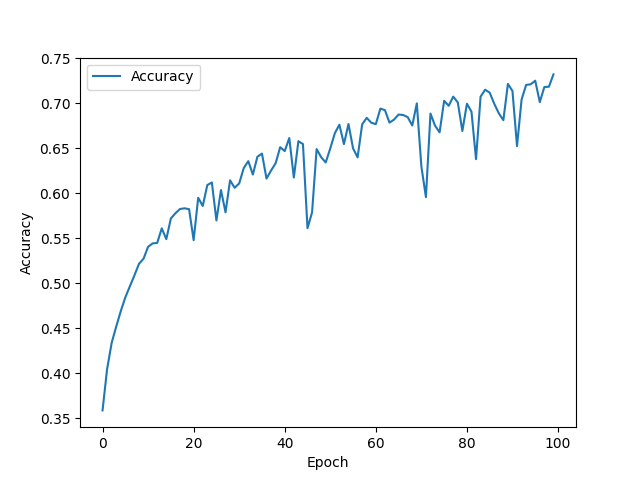
\includegraphics[width=\textwidth]{img/Q2/Acc.png}
    \end{subfigure}
    \hfill
    \begin{subfigure}[t]{0.45\linewidth}
        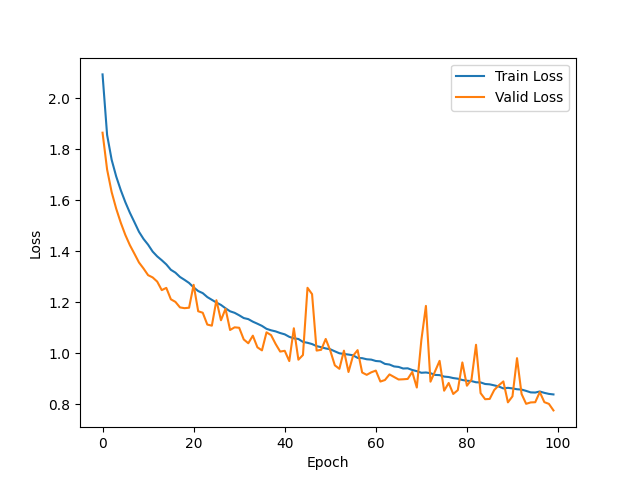
\includegraphics[width=\textwidth]{img/Q2/Loss.png}
    \end{subfigure}
    \hfill
\end{figure}

\section{}
在AdamW优化器下,使用ReLU激活函数与Batch Normalization,输出的结果如下:
\begin{figure}[H]
    \hfill
    \begin{subfigure}[t]{0.45\linewidth}
        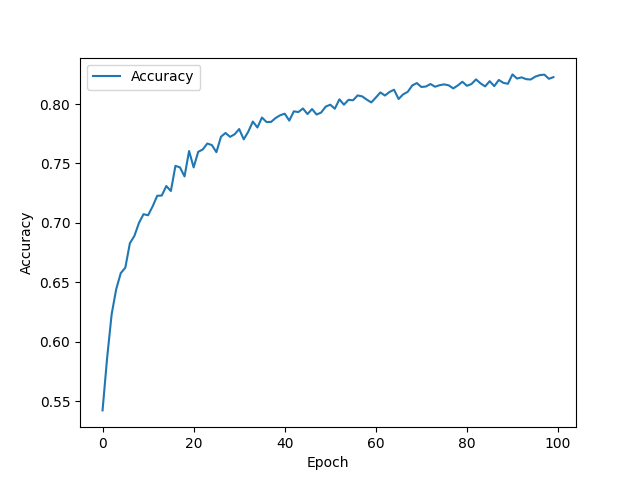
\includegraphics[width=\textwidth]{img/Q3/Acc.png}
    \end{subfigure}
    \hfill
    \begin{subfigure}[t]{0.45\linewidth}
        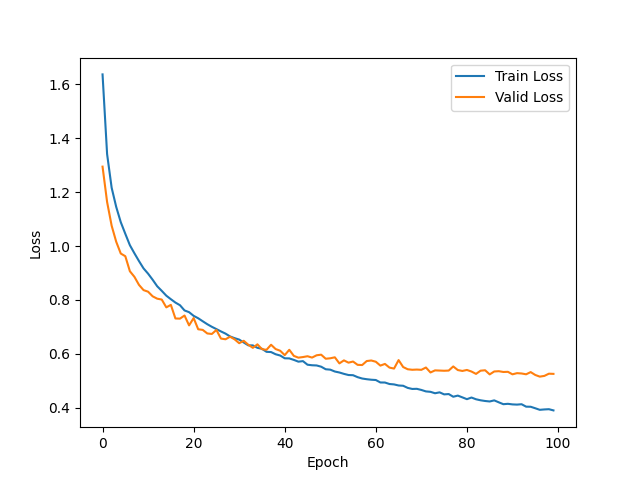
\includegraphics[width=\textwidth]{img/Q3/Loss.png}
    \end{subfigure}
    \hfill
\end{figure}

\section{}
\subsection{}
仍旧使用$\tanh$作为激活函数,SGD优化器:
\begin{figure}[H]
    \hfill
    \begin{subfigure}[t]{0.45\linewidth}
        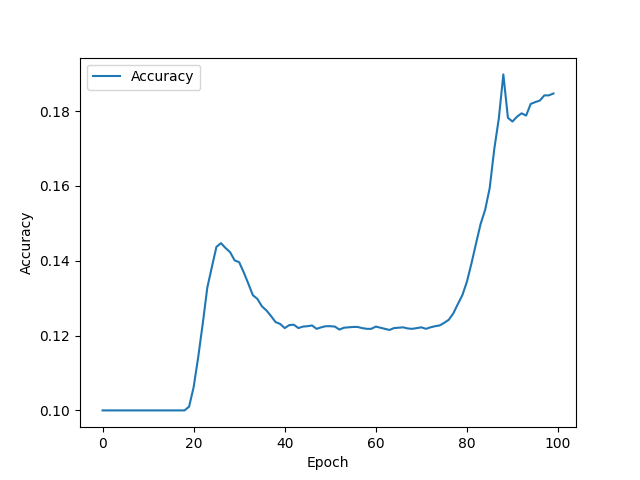
\includegraphics[width=\textwidth]{img/Q4/1/Acc.png}
    \end{subfigure}
    \hfill
    \begin{subfigure}[t]{0.45\linewidth}
        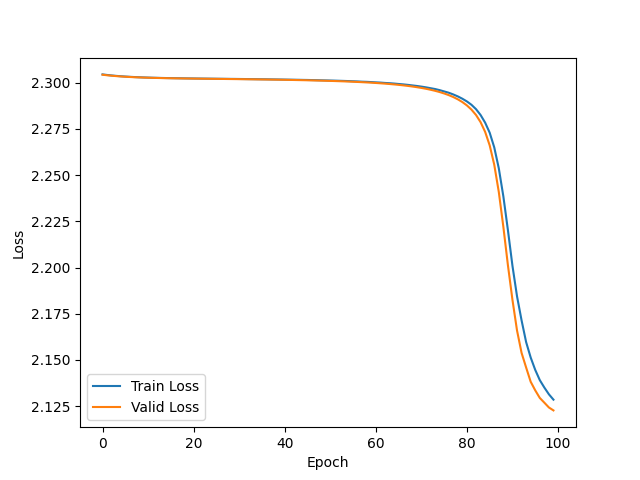
\includegraphics[width=\textwidth]{img/Q4/1/Loss.png}
    \end{subfigure}
    \hfill
\end{figure}
\subsection{}
将激活函数更改为ReLU函数,并使用BatchNorm,使用SGD:
\begin{figure}[H]
    \hfill
    \begin{subfigure}[t]{0.45\linewidth}
        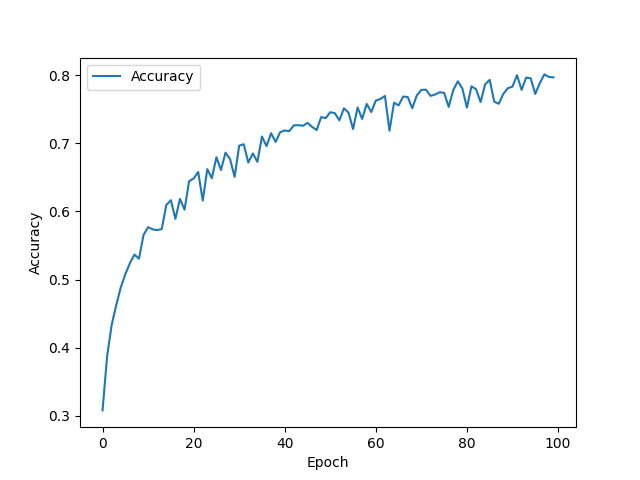
\includegraphics[width=\textwidth]{img/Q4/2/Acc.png}
    \end{subfigure}
    \hfill
    \begin{subfigure}[t]{0.45\linewidth}
        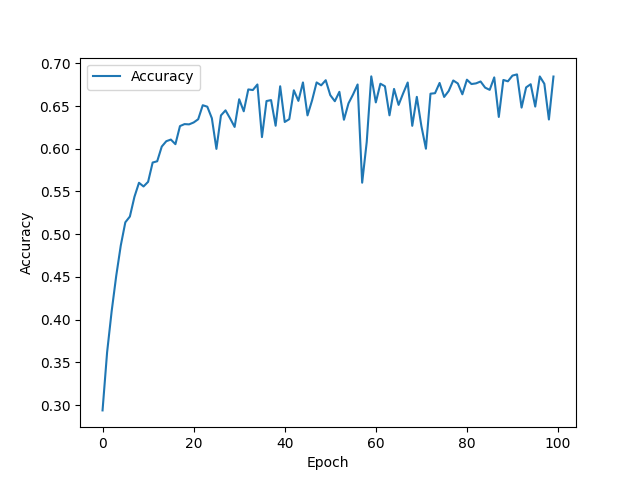
\includegraphics[width=\textwidth]{img/Q4/2/Loss.png}
    \end{subfigure}
    \hfill
\end{figure}
\subsection{}
在AdamW优化器下,使用ReLU激活函数与Batch Normalization,输出的结果如下:
\begin{figure}[H]
    \hfill
    \begin{subfigure}[t]{0.45\linewidth}
        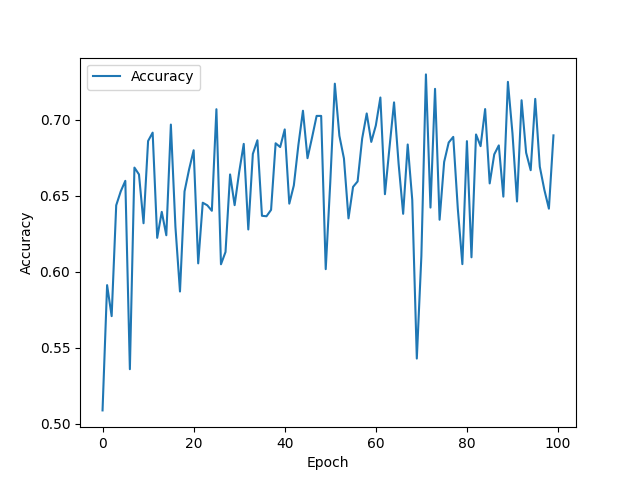
\includegraphics[width=\textwidth]{img/Q4/3/Acc.png}
    \end{subfigure}
    \hfill
    \begin{subfigure}[t]{0.45\linewidth}
        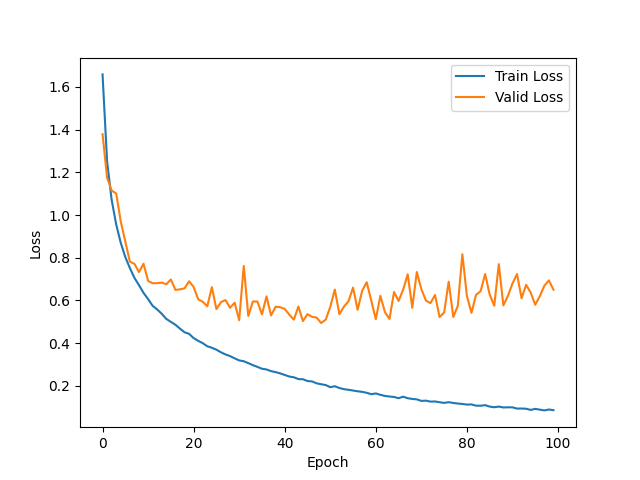
\includegraphics[width=\textwidth]{img/Q4/3/Loss.png}
    \end{subfigure}
    \hfill
\end{figure}

\section{}
\begin{enumerate}
    \item 请根据结果分析 ReLU 和 tanh 激活函数的表现.
    
    由于实验1与实验2同时更改了激活函数与是否增加Batch Normalization,我们无法直接从实验结果中通过对比得出ReLU与tanh到底哪个表现更好。不过从理论上进行分析,ReLU激活函数在当前任务中的表现应当会优于tanh激活函数。这是由于ReLU激活函数不存在梯度消失问题,能够使网络快速收敛,无论网络深浅;而tanh函数容易陷入饱和区、导致梯度消失,使得网络收敛速度大幅降低,特别是在深层次网络中这一现象更加明显;因此,在CNN架构中,ReLU激活函数表现应该会优于tanh。

    \item 请根据结果分析 BatchNorm 的作用.
    
    由于实验1与实验2同时更改了激活函数与是否增加Batch Normalization,我们无法直接从实验结果中通过对比看出BatchNorm的作用。不过从理论上进行分析,BatchNorm可以使网络中每一层的数据分布均值为0、方差为1,这样神经元输出值不会太大,加强了网络稳定性,同时防止出现梯度爆炸(或梯度消失),使网络能够较快收敛;此外,Batch Normalization可以使相同batch中的所有样本相互关联,加强了泛化性,避免过拟合。

    \item 请根据结果分析更换优化器的效果.
    
    从实验2、3的结果对比中可以看出,使用SGD优化器会导致测试准确率与训练、测试损失出现明显震荡,而更换了AdamW优化器以后准确率曲线与损失曲线都更加平滑。SGD优化器容易出现振荡是由于它会导致梯度值相差较大的方向上优化步长差异也大,致使梯度值大的方向上产生振荡;而Adam优化器可以根据不同参数梯度值自适应地调整各个方向的优化步长大小,以使各个方向都能同时得到有效且合理的优化。

    \item 请根据你的结果分析模型是否出现了过拟合,如有,请在图像中指出在哪里出现了过拟合。如无,请给出你判断的原因.
    
    通过训练/测试损失曲线以及测试准确率曲线可知,实验4的第3部分出现了过拟合现象,发生在epoch 35附近。判断依据:训练损失持续降低,而测试损失不再降低甚至开始升高且出现巨幅振荡,测试准确率也不再增加。
\end{enumerate}

\section*{程序源代码}
\lstinputlisting[style=python]{../CIFAR10_playground.py}
\end{document}